% topic1.tex -- Topic 1: Charged particles, conductors and electric and magnetic fields, Q1-18.
% Directions: right = +x, up the page = +y, out of the page = +z.
\firsttopictitle{Topic 1 - Charged Particles in Electric and Magnetic Fields}

% ---- Q1 (what does NOT change the magnetic force)
\begin{quizq}{}
A proton moves at right angles to a uniform magnetic field. Which change would NOT change the size of
the magnetic force on the particle?
\opts{Doubling the strength of the magnetic field}{Doubling the speed of the particle}
  {Replacing the proton with an electron moving at the same speed}
  {Replacing the proton with an alpha particle moving at the same speed}
\end{quizq}

% ---- Q2 (which field can change the kinetic energy)
\Needspace{12\baselineskip}
\begin{quizq}{}
A proton enters a region of space with a velocity at right angles to the field in that region.
Which type of field could change the kinetic energy of the proton?
\opts{A magnetic field only}{An electric field only}{Both an electric field and a magnetic field}
  {Neither type of field}
\end{quizq}

% ---- Q3 (E between plates)
\Needspace{22\baselineskip}
\begin{quizq}{}
The diagram shows two parallel charged plates \qty{2.0}{mm} apart.
\begin{center}
  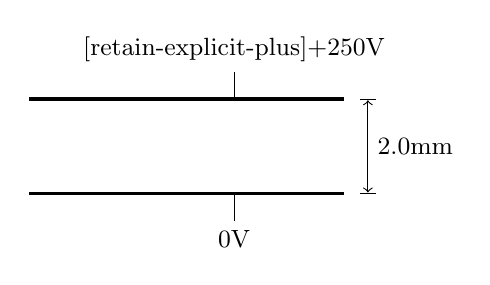
\begin{tikzpicture}
    \draw[line width=1.2pt] (0,1.2) -- (4,1.2); \draw[line width=1.2pt] (0,0) -- (4,0);
    \draw (2.6,1.2) -- (2.6,1.55) node[above, font=\small] {\qty[retain-explicit-plus]{+250}{V}};
    \draw (2.6,0) -- (2.6,-0.35) node[below, font=\small] {\qty{0}{V}};
    \draw[|<->|, line width=0.4pt] (4.3,0) -- (4.3,1.2) node[midway, right, font=\small] {\qty{2.0}{mm}};
  \end{tikzpicture}
\end{center}
What is the magnitude of the electric field between the plates, in \si{V.m^{-1}}?
\opts{\num{8.0e-6}}{0.50}{125}{\num{1.25e5}}
\end{quizq}

% ---- Q4 (radius of a proton's path)
\Needspace{12\baselineskip}
\begin{quizq}{}
A proton moves at \qty{3.0e6}{m.s^{-1}} at right angles to a uniform magnetic field of
\qty{0.20}{T}. What is the radius of its circular path?
\opts{\qty{8.5e-5}{m}}{\qty{0.16}{m}}{\qty{6.4}{m}}{\qty{4.7e5}{m}}
\end{quizq}

% ---- Q5 (direction of B from an electron's path)
\Needspace{24\baselineskip}
\begin{quizq}{}
An electron moving to the right enters a region of uniform magnetic field (shaded) and follows the
curved path shown.
\begin{center}
  \begin{tikzpicture}
    \fill[black!8] (1.5,-0.3) rectangle (4.5,2.4); \draw[guide] (1.5,-0.3) rectangle (4.5,2.4);
    \node[font=\small] at (3.9,0.1) {$B = \;?$};
    \draw[->, line width=0.7pt] (0,0) -- (1.0,0); \fill (0,0) circle (2pt) node[left, font=\small] {$e^-$};
    \draw[line width=0.8pt, dash pattern=on 3pt off 2pt] (1.0,0) -- (1.5,0) arc (-90:0:1.6);
  \end{tikzpicture}
\end{center}
What is the direction of the magnetic field?
\opts{Up the page}{Down the page}{Into the page}{Out of the page}
\end{quizq}

% ---- Q6 (velocity selector entered at twice the speed)
\Needspace{16\baselineskip}
\begin{quizq}{}
A positive ion moves at speed $v$ in a straight line through a region of crossed electric and magnetic
fields, without being deflected. An identical ion then enters the same region in the same direction at
speed $2v$. Which statement is correct?
\opts{The second ion also passes through without being deflected.}
  {The second ion is deflected in the direction of the electric force.}
  {The second ion is deflected in the direction of the magnetic force.}
  {Both the electric force and the magnetic force on the second ion are doubled.}
\end{quizq}

% ---- Q7 (radius when v doubles and B halves)
\Needspace{12\baselineskip}
\begin{quizq}{}
A charged particle moves in a circle of radius $r$ in a uniform magnetic field. The speed of the
particle is doubled and the magnetic field strength is halved. What is the new radius?
\opts{$\dfrac{r}{4}$}{$r$}{$2r$}{$4r$}
\end{quizq}

% ---- Q8 (largest magnetic force)
\Needspace{30\baselineskip}
\begin{quizq}{}
In which situation does the magnetic field exert the greatest force on the proton (the black dot)? All the
magnetic fields have the same strength.
\gridopts{%
  \begin{tikzpicture}
    \foreach \y in {0,2.0} \draw[->, line width=0.5pt] (0,\y) -- (3,\y); \node[right, font=\small] at (3,2.0) {$B$};
    \fill (0.9,0.6) circle (2.5pt); \draw[->, line width=0.8pt] (0.9,0.6) -- (0.9,1.4);
    \node[right, font=\small] at (1.0,1.1) {\qty{50}{m.s^{-1}}};
  \end{tikzpicture}}
  {%
  \begin{tikzpicture}
    \foreach \y in {0,2.0} \draw[->, line width=0.5pt] (0,\y) -- (3,\y); \node[right, font=\small] at (3,2.0) {$B$};
    \fill (0.6,0.6) circle (2.5pt); \draw[->, line width=0.8pt] (0.6,0.6) -- ++(30:0.9);
    \draw[guide] (0.6,0.6) -- (1.7,0.6); \draw (1.1,0.6) arc (0:30:0.5); \node[font=\scriptsize] at (1.35,0.4) {\ang{30}};
    \node[right, font=\small] at (1.45,1.15) {\qty{80}{m.s^{-1}}};
  \end{tikzpicture}}
  {%
  \begin{tikzpicture}
    \foreach \y in {0,2.0} \draw[->, line width=0.5pt] (0,\y) -- (3,\y); \node[right, font=\small] at (3,2.0) {$B$};
    \fill (0.6,0.9) circle (2.5pt); \draw[->, line width=0.8pt] (0.6,0.9) -- (1.5,0.9);
    \node[right, font=\small] at (1.55,0.9) {\qty{100}{m.s^{-1}}};
  \end{tikzpicture}}
  {%
  \begin{tikzpicture}
    \foreach \y in {0,2.0} \draw[->, line width=0.5pt] (0,\y) -- (3,\y); \node[right, font=\small] at (3,2.0) {$B$};
    \fill (0.6,0.6) circle (2.5pt); \draw[->, line width=0.8pt] (0.6,0.6) -- ++(45:0.9);
    \draw[guide] (0.6,0.6) -- (1.7,0.6); \draw (1.1,0.6) arc (0:45:0.5); \node[font=\scriptsize] at (1.35,0.4) {\ang{45}};
    \node[right, font=\small] at (1.3,1.35) {\qty{60}{m.s^{-1}}};
  \end{tikzpicture}}
\end{quizq}

% ---- Q9 (proton instead of electron: deflection on a screen)
\Needspace{26\baselineskip}
\begin{quizq}{}
An electron is fired in a vacuum towards a screen. With no electric field, it hits the screen at $P$.
A uniform electric field is then turned on, and a second electron, fired from the same place with the
same velocity, hits the screen at $Q$.
\begin{center}
  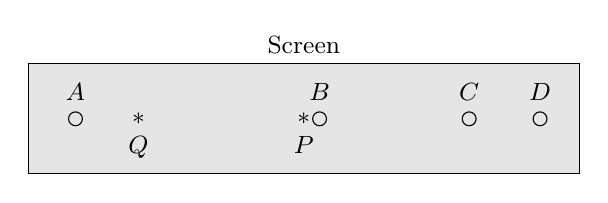
\begin{tikzpicture}
    \fill[black!10] (0,0) rectangle (7,1.4); \draw (0,0) rectangle (7,1.4);
    \node[above, font=\small] at (3.5,1.4) {Screen};
    \foreach \x/\l in {0.6/A, 3.7/B, 5.6/C, 6.5/D} {\draw (\x,0.7) circle (2.5pt); \node[above=3pt, font=\small] at (\x,0.7) {$\l$};}
    \node[font=\small] at (1.4,0.7) {$*$}; \node[below=3pt, font=\small] at (1.4,0.7) {$Q$};
    \node[font=\small] at (3.5,0.7) {$*$}; \node[below=3pt, font=\small] at (3.5,0.7) {$P$};
  \end{tikzpicture}
\end{center}
With the field still on, a proton is fired from the same place with the same velocity. Where does the
proton hit the screen?
\opts{$A$}{$B$}{$C$}{$D$}
\end{quizq}

% ---- Q10 (kinetic energy gained over a fixed distance)
\Needspace{14\baselineskip}
\begin{quizq}{}
A positively charged particle starts from rest at point $X$ between two parallel plates and moves a
fixed distance to point $Y$. Its gain in kinetic energy is $W$.

The voltage across the plates is then doubled AND the distance between the plates is doubled. The
particle again moves from rest from $X$ to $Y$. What is its gain in kinetic energy now?
\opts{$\dfrac{W}{2}$}{$W$}{$2W$}{$4W$}
\end{quizq}

% ---- Q11 (velocity selector: directions for a proton)
\Needspace{28\baselineskip}
\begin{quizq}{}
A proton moves to the right between two charged plates and is deflected as shown.
\begin{center}
  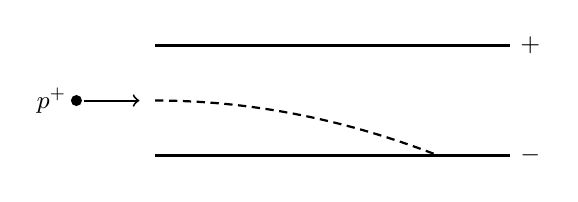
\begin{tikzpicture}
    \draw[line width=1.2pt] (1,1.4) -- (5.5,1.4) node[right, font=\small] {$+$};
    \draw[line width=1.2pt] (1,0) -- (5.5,0) node[right, font=\small] {$-$};
    \fill (0,0.7) circle (2pt) node[left, font=\small] {$p^+$}; \draw[->, line width=0.7pt] (0.1,0.7) -- (0.8,0.7);
    \draw[line width=0.8pt, dash pattern=on 3pt off 2pt, domain=0:3.6, samples=30, smooth] plot ({1+\x}, {0.7-0.054*\x*\x});
  \end{tikzpicture}
\end{center}
A magnetic field is then added, so that a second proton with the same velocity passes through
undeflected. Which row of the table gives the directions of the two fields?
\begin{center}
  \renewcommand\arraystretch{1.7}
  \begin{tabular}{@{}p{10mm}|>{\centering\arraybackslash}p{50mm}|>{\centering\arraybackslash}p{40mm}|}
    \cline{2-3}
    & \textit{Electric field} & \textit{Magnetic field}\\ \cline{2-3}
    A. & Towards the top of the page & Into the page\\ \cline{2-3}
    B. & Towards the top of the page & Out of the page\\ \cline{2-3}
    C. & Towards the bottom of the page & Into the page\\ \cline{2-3}
    D. & Towards the bottom of the page & Out of the page\\ \cline{2-3}
  \end{tabular}
\end{center}
\end{quizq}

% ---- Q12 (velocity selector: B for electrons)
\Needspace{24\baselineskip}
\begin{quizq}{}
A beam of electrons travels at \qty{4.0e6}{m.s^{-1}} between two parallel plates \qty{2.0}{mm} apart.
The top plate is at \qty[retain-explicit-plus]{+800}{V} and the bottom plate is at \qty{0}{V}.
\begin{center}
  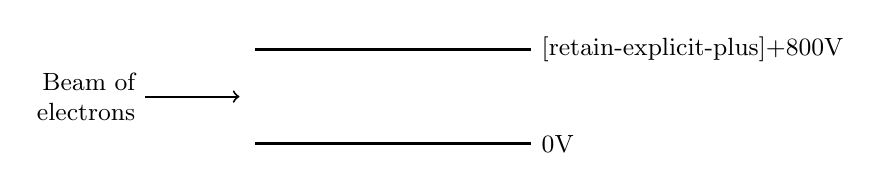
\begin{tikzpicture}
    \draw[line width=1.2pt] (1,1.2) -- (4.5,1.2) node[right, font=\small] {\qty[retain-explicit-plus]{+800}{V}};
    \draw[line width=1.2pt] (1,0) -- (4.5,0) node[right, font=\small] {\qty{0}{V}};
    \draw[->, line width=0.7pt] (-0.4,0.6) -- (0.8,0.6); \node[left, font=\small, align=right] at (-0.4,0.6) {Beam of\\electrons};
  \end{tikzpicture}
\end{center}
A magnetic field is applied so that the electrons continue in a straight line. What are the magnitude
and direction of this magnetic field?
\opts{\qty{0.10}{T} into the page}{\qty{0.10}{T} out of the page}{\qty{10}{T} into the page}
  {\qty{10}{T} out of the page}
\end{quizq}

% ---- Q13 (direction of motion through crossed fields: electron)
\Needspace{24\baselineskip}
\begin{quizq}{}
The diagram shows a region with a uniform electric field (between the charged plates) and a uniform
magnetic field out of the page. An electron moves through the region at a constant velocity.
\begin{center}
  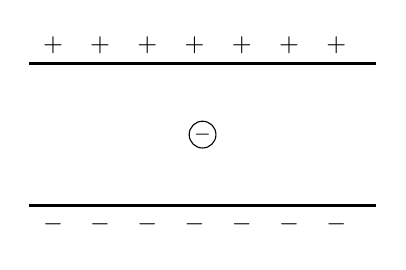
\begin{tikzpicture}
    \draw[line width=1.2pt] (0,1.8) -- (4.4,1.8); \foreach \x in {0.3,0.9,...,4.2} \node[above, font=\small] at (\x,1.8) {$+$};
    \draw[line width=1.2pt] (0,0) -- (4.4,0); \foreach \x in {0.3,0.9,...,4.2} \node[below, font=\small] at (\x,0) {$-$};
    \fieldout{0.4}{0.4}{4.0}{1.4}{0.5}
    \fill[white] (2.2,0.9) circle (0.17); \draw (2.2,0.9) circle (0.17); \node[font=\scriptsize] at (2.2,0.9) {$-$};
  \end{tikzpicture}
\end{center}
In which direction is the electron moving?
\opts{Up the page}{Down the page}{To the left}{To the right}
\end{quizq}

% ---- Q14 (speed after acceleration through 2.0 kV)
\Needspace{12\baselineskip}
\begin{quizq}{}
An electron starts from rest and is accelerated through a potential difference of \qty{2.0}{kV}.
What is its final speed?
\opts{\qty{6.2e5}{m.s^{-1}}}{\qty{1.9e7}{m.s^{-1}}}{\qty{2.7e7}{m.s^{-1}}}{\qty{7.0e14}{m.s^{-1}}}
\end{quizq}

% ---- Q15 (gravitational field vs electric field when the charge is doubled)
\Needspace{36\baselineskip}
\begin{quizq}{}
Two identical charged particles are launched horizontally with the same velocity $u$. One moves in a
uniform gravitational field (Figure I), the other in a uniform electric field (Figure II, gravity
negligible). $X$ and $Y$ are their landing points.
\begin{center}
  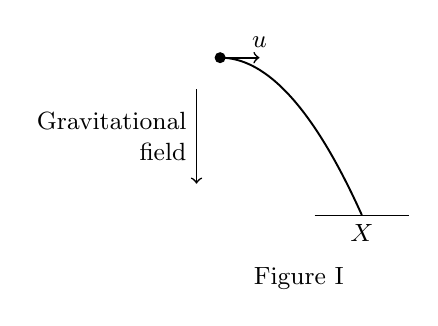
\begin{tikzpicture}
    \draw[->, line width=0.6pt] (-0.3,1.6) -- (-0.3,0.4) node[midway, left, font=\small, align=right] {Gravitational\\field};
    \fill (0,2) circle (2pt); \draw[->, line width=0.6pt] (0,2) -- (0.5,2) node[above, font=\small] {$u$};
    \draw[line width=0.7pt, domain=0:1.8, samples=30, smooth] plot (\x, {2-0.617*\x*\x});
    \draw (1.2,0) -- (2.4,0); \node[below, font=\small] at (1.8,0) {$X$};
    \node[font=\small] at (1,-0.8) {Figure I};
  \end{tikzpicture}\hspace{20mm}%
  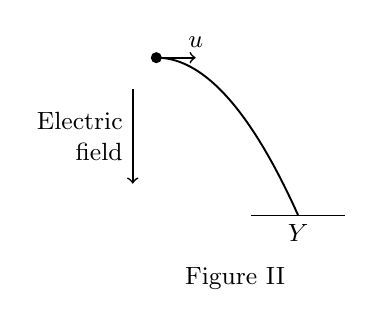
\begin{tikzpicture}
    \draw[->, line width=0.6pt] (-0.3,1.6) -- (-0.3,0.4) node[midway, left, font=\small, align=right] {Electric\\field};
    \fill (0,2) circle (2pt); \draw[->, line width=0.6pt] (0,2) -- (0.5,2) node[above, font=\small] {$u$};
    \draw[line width=0.7pt, domain=0:1.8, samples=30, smooth] plot (\x, {2-0.617*\x*\x});
    \draw (1.2,0) -- (2.4,0); \node[below, font=\small] at (1.8,0) {$Y$};
    \node[font=\small] at (1,-0.8) {Figure II};
  \end{tikzpicture}
\end{center}
The charge on each particle is doubled (the masses stay the same) and they are launched again with
the same velocity $u$. Which row of the table describes the new landing points?
\begin{center}
  \renewcommand\arraystretch{1.7}
  \begin{tabular}{@{}p{10mm}|>{\centering\arraybackslash}p{48mm}|>{\centering\arraybackslash}p{48mm}|}
    \cline{2-3}
    & \textit{Gravitational field (Figure I)} & \textit{Electric field (Figure II)}\\ \cline{2-3}
    A. & Same point $X$ & Closer to the start than $Y$\\ \cline{2-3}
    B. & Closer to the start than $X$ & Same point $Y$\\ \cline{2-3}
    C. & Same point $X$ & Further from the start than $Y$\\ \cline{2-3}
    D. & Closer to the start than $X$ & Closer to the start than $Y$\\ \cline{2-3}
  \end{tabular}
\end{center}
\end{quizq}

% ---- Q16 (electric field that halves the drop)
\Needspace{26\baselineskip}
\begin{quizq}{}
A particle of mass $m$ and positive charge $q$ is fired horizontally into a vacuum chamber. Under
gravity alone, it falls \qty{10}{cm} while it travels a horizontal distance $d$.
\begin{center}
  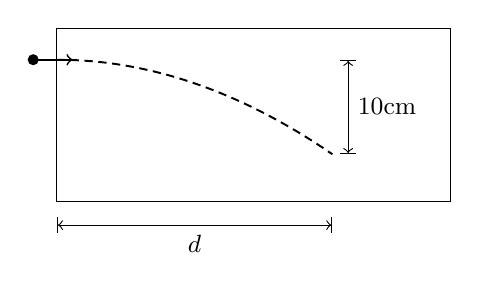
\begin{tikzpicture}
    \draw (0,0) rectangle (5,2.2);
    \fill (-0.3,1.8) circle (2pt); \draw[->, line width=0.6pt] (-0.3,1.8) -- (0.2,1.8);
    \draw[line width=0.7pt, dash pattern=on 3pt off 2pt, domain=0:3.5, samples=30, smooth] plot (\x, {1.8-0.098*\x*\x});
    \draw[|<->|, line width=0.4pt] (3.7,1.8) -- (3.7,0.6) node[midway, right, font=\small] {\qty{10}{cm}};
    \draw[|<->|, line width=0.4pt] (0,-0.3) -- (3.5,-0.3) node[midway, below, font=\small] {$d$};
  \end{tikzpicture}
\end{center}
A uniform vertical electric field is then turned on. The particle, fired in the same way, now falls only
\qty{5}{cm} over the same horizontal distance $d$. What is the magnitude of the electric field?
\opts{$\dfrac{mg}{2q}$}{$\dfrac{mg}{q}$}{$\dfrac{3mg}{2q}$}{$\dfrac{2mg}{q}$}
\end{quizq}

% ---- Q17 (electron beam beside a current-carrying wire)
\Needspace{22\baselineskip}
\begin{quizq}{}
A beam of electrons travels parallel to a long straight wire, in the same direction as the
conventional current $I$ in the wire, as shown.
\begin{center}
  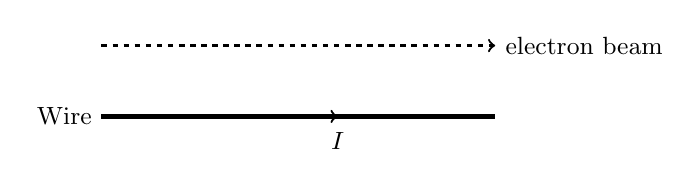
\begin{tikzpicture}
    \draw[line width=1.6pt] (0,0) -- (5,0); \draw[->, line width=0.8pt] (2,0.0) -- (3,0.0) node[below=2pt, font=\small] {$I$};
    \draw[line width=0.8pt, dash pattern=on 2pt off 2pt, ->] (0,0.9) -- (5,0.9) node[right, font=\small] {electron beam};
    \node[left, font=\small] at (0,0) {Wire};
  \end{tikzpicture}
\end{center}
How is the electron beam deflected?
\opts{Towards the wire}{Away from the wire}{Into the page}{It is not deflected}
\end{quizq}

% ---- Q18 (field switched on halfway down)
\Needspace{40\baselineskip}
\begin{quizq}{}
A small positively charged mass falls from rest in an evacuated chamber, between two vertical
parallel plates. At first the plates are not charged. When the mass has fallen halfway, the plates are
connected to a power supply so that the left plate is positive and the right plate is negative.
Which diagram best shows the path of the mass?
\gridopts{%
  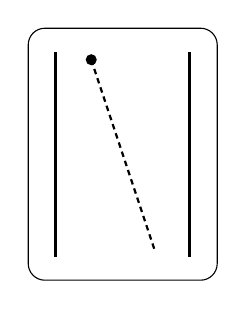
\begin{tikzpicture}
    \draw[rounded corners=6pt] (0,0) rectangle (2.4,3.2); \draw[line width=1pt] (0.35,0.3) -- (0.35,2.9); \draw[line width=1pt] (2.05,0.3) -- (2.05,2.9);
    \fill (0.8,2.8) circle (2pt); \draw[line width=0.8pt, dash pattern=on 2pt off 1.5pt] (0.8,2.8) -- (1.6,0.4);
  \end{tikzpicture}}
  {%
  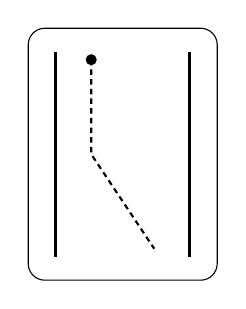
\begin{tikzpicture}
    \draw[rounded corners=6pt] (0,0) rectangle (2.4,3.2); \draw[line width=1pt] (0.35,0.3) -- (0.35,2.9); \draw[line width=1pt] (2.05,0.3) -- (2.05,2.9);
    \fill (0.8,2.8) circle (2pt); \draw[line width=0.8pt, dash pattern=on 2pt off 1.5pt] (0.8,2.8) -- (0.8,1.6) -- (1.6,0.4);
  \end{tikzpicture}}
  {%
  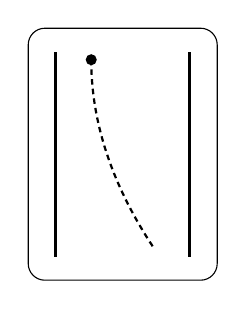
\begin{tikzpicture}
    \draw[rounded corners=6pt] (0,0) rectangle (2.4,3.2); \draw[line width=1pt] (0.35,0.3) -- (0.35,2.9); \draw[line width=1pt] (2.05,0.3) -- (2.05,2.9);
    \fill (0.8,2.8) circle (2pt); \draw[line width=0.8pt, dash pattern=on 2pt off 1.5pt, domain=0:2.4, samples=30, smooth] plot ({0.8+0.139*\x*\x}, {2.8-\x});
  \end{tikzpicture}}
  {%
  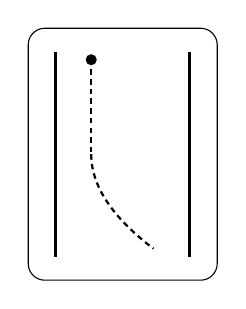
\begin{tikzpicture}
    \draw[rounded corners=6pt] (0,0) rectangle (2.4,3.2); \draw[line width=1pt] (0.35,0.3) -- (0.35,2.9); \draw[line width=1pt] (2.05,0.3) -- (2.05,2.9);
    \fill (0.8,2.8) circle (2pt); \draw[line width=0.8pt, dash pattern=on 2pt off 1.5pt] (0.8,2.8) -- (0.8,1.6);
    \draw[line width=0.8pt, dash pattern=on 2pt off 1.5pt, domain=0:1.2, samples=30, smooth] plot ({0.8+0.55*\x*\x}, {1.6-\x});
  \end{tikzpicture}}
\end{quizq}
